\documentclass[11pt, a4paper, german]{article}
%\usepackage[top=2cm, bottom=2cm]{geometry}
\pagestyle{plain}

\usepackage[german]{babel}
\usepackage{amsmath}
\usepackage{amsthm}
\usepackage{amssymb}
\usepackage{graphicx}
\usepackage{tikz}
\usepackage[utf8]{inputenc}
\usepackage{caption}
\usepackage{subcaption}
\usepackage[colorlinks=true, pdfborder={0 0 0}, linkcolor=blue, citecolor=blue]{hyperref}

\newcommand{\HRule}{\rule{\linewidth}{0.5mm}}
\setlength{\parindent}{0cm}

\begin{document}
\begin{titlepage}

\begin{center}


% Oberer Teil der Titelseite:

\textsc{\LARGE Projektgruppe Angewandte Softwaretechnologie}\\[1.5cm]

\textsc{\Large Sommersemester 2015}\\[0.5cm]

\HRule \\[0.4cm] { \huge \bfseries DLVC Taverne}\\[0.2cm]
{\large \bfseries Ein Handbuch}\\[0.4cm]

\HRule \\[1.5cm]

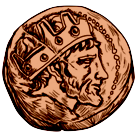
\includegraphics[width=0.6\textwidth]{./Logo3_1.png}\\[1cm]

\begin{minipage}{0.4\textwidth} \begin{flushleft} \large \emph{Author:}\\ Projektgruppe DLVC Taverne \end{flushleft} \end{minipage} \hfill \begin{minipage}{0.4\textwidth} \begin{flushright} \large \emph{Supervisor:} \\ Günther Kniesel \end{flushright} \end{minipage}

\vfill

{\large \today}

\end{center}

\end{titlepage}
\clearpage

\tableofcontents
\pagebreak

\section{Allgemeine Informationen}
Die Zielsetzung von 'DLVC Taverne' ist es, Spielleitern im Pen\&Paper-Rollenspiel 'Die Legenden von Cystaron' (DLVC) ihre Aufgabe zu erleichtern. Insbesondere im Kampf sollen langwierige Würfeleien und Rechnungen vonseiten des Spielleiters vermieden werden.
\subsection{Hinweis}
Dieses Handbuch geht davon aus, dass dem Leser die Regeln von DLVC bekannt sind. 
\subsection{Arbeitsgruppe}
Das Programm 'DLVC Taverne' ist 2015 im Rahmen der Projektgruppe 'Angewandte Softwaretechnologie' unter der Leitung von Dr. Kniesel entstanden. Die Entwickler waren:
\begin{itemize}
	\item[] Britta Heymann
	\item[] Andreas Kofer
	\item[] Nooshin Naghavi
	\item[] Boris Prochnau
\end{itemize}

\newpage
\section{Das Hauptmenü}
Das Hauptmenü besteht aus zwei vertikal getrennten Bereichen, den Buttons für die Hauptfunktionen und der Gruppenauswahl (siehe Abb. \ref{fig:Hauptmenue1}). Außerdem findet sich (wie auf fast jedem Fenster) ein Hilfe Button am rechten unteren Rand, welcher über das aktuelle Fenster informieren kann.
\begin{figure}
\centering
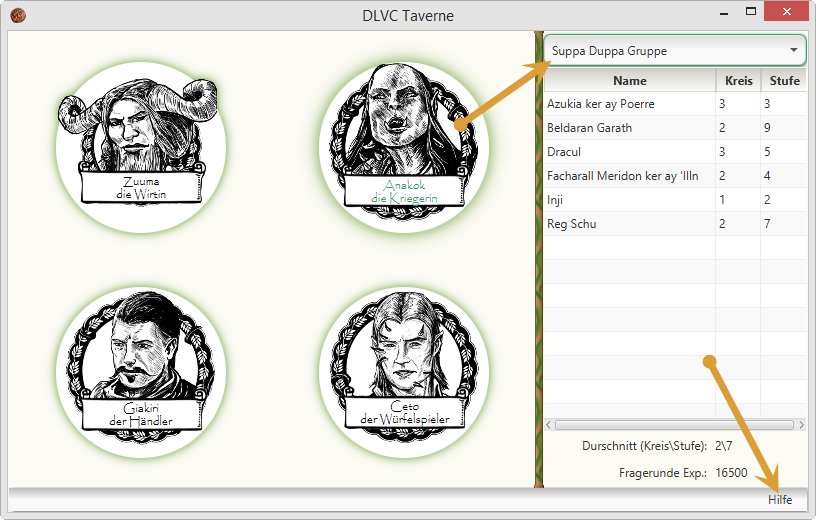
\includegraphics[width=1\linewidth]{Bilder/Hauptmenue1}
\caption{Hauptmenü}
\label{fig:Hauptmenue1}
\end{figure}

\subsection{Button Bereich}
%\textbf{Button Bereich:}\\
Im linken Bereich finden sich vier Buttons, um auf die Grundfunktionen des Programm zuzugreifen.
\begin{itemize}
	\item[] \textbf{Charaktermanager}: Hier können Spielercharaktere und Nichtspieler-Charakter-Typen angelegt, sowie Abenteuergruppen verwaltet werden.
	\item[] \textbf{Kampf}: Führt zu einer Teilnehmerauswahl für die Teilnehmer des Kampfes (Spieler und Gegner). Anschließend kann ein Kampfhelfer für den Kampf gestartet werden.
	\item[] \textbf{Händler}: Hier können alle Gegenstände und Ausrüstungsteile erstellt, gesucht und anderweitig verwaltet werden.
	\item[] \textbf{Würfeln}: Hier können diverse Würfelwürfe simuliert werden.
\end{itemize}

\subsection{Gruppenauswahl}\label{subsection:gruppenauswahl}
Im rechten Bereich findet sich die Gruppenauswahl. Jede zuvor im Charaktermanger zusammengestellte Gruppe kann in Combo-Box ganz oben ausgewählt werden, woraufhin alle Mitglieder mit Kreis und Level angezeigt werden.\\
Die Auswahl einer Gruppe im Hauptmenü führt dazu, dass diese die Standardgruppe in der Abenteuerverwaltung und bei Kämpfen ist.

\newpage

\section{Der Charaktermanager}
Um den Kampfhelfer zu nutzen, müssen 'DLVC Taverne' Spielercharaktere und Nichtspieler-Typen bekannt sein. Dafür ist der Charaktermanager zuständig. Er teilt sich in die drei Tabs \textbf{Gruppen}, \textbf{Spielercharaktere} und \textbf{Nichtspieler-Typen}.

\subsection{Der Gruppenmanager}
Der Gruppenmanager ermöglicht das Speichern von Abenteuergruppen. Diese können dann schnell bei Neustart wiederverwendet und angepasst werden.\\
Große Vorteile sind dass man im Kampf standardmäßig die entsprechenden Mitglieder der Gruppe als Teilnehmer hat und durch einmalige Auswahl im Hauptmenü stets verfolgen kann welche Stufe die Spieler haben und bemerken wenn sie geändert werden müssen (siehe Abschnitt \ref{subsection:gruppenauswahl}).\\
\begin{figure}
\centering
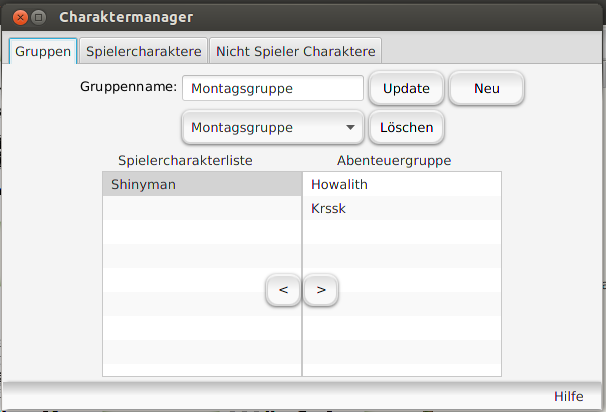
\includegraphics[width=1\linewidth]{Bilder/Gruppenmanager}
\caption{Der Gruppenmanager}
\label{fig:Gruppenmanager}
\end{figure}

Der Gruppenmanager besteht im wesentlichen aus zwei Listen und dem oberen Bereich zum Anpassen der Gruppennamen.\\

\textbf{Anlegen neuer Gruppen}: Dazu muss ein Name in das obere Textfeld geschrieben und mit dem Button '\textbf{Neu}' oder mit der 'Enter'-Taste bestätigt werden.\\

\textbf{Ändern einer Gruppe}: Existieren bereits Gruppen, so kann man sie in der unter dem Textfeld liegenden Box auswählen. Der Name erscheint dann im Textfeld und kann editiert und mit einem Klick auf den Button '\textbf{Update}' gespeichert werden. \\

\textbf{Löschen einer Gruppe}: Mit dem '\textbf{Löschen}'-Button wird die selektierte Gruppe gelöscht. \textit{Hinweis}: Dies löscht nur die Zuordnungen der Spielercharaktere zu der Gruppe, nicht die Spielercharaktere selbst.\\

Um Spielercharaktere zu einer Gruppe hinzuzufügen oder zu entfernen, muss die entsprechende Gruppe selektiert werden. Durch Klicken auf die Pfeilbuttons wird die neue Aufteilung herbeigeführt und direkt abgespeichert.

\subsection{Der Spielercharaktermanager}\label{subsection:Spielercharaktermanager}
Im Spielercharaktermanager werden die kampfrelevanten Eigenschaften von Spielercharakteren abgespeichert. 
Er ist dafür in die drei Untertabs 'Details', 'Waffen\&Fähigkeiten' und 'Ausrüstung' aufgeteilt.\\
\begin{figure}[h!]
\centering
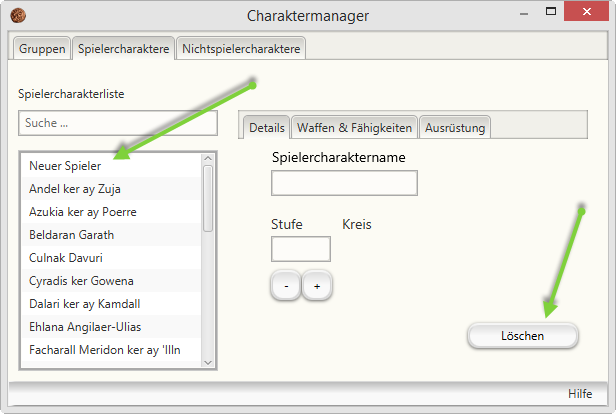
\includegraphics[width=1\linewidth]{Bilder/Charaktermanager1}
\caption{Neuen Spieler auswählen und Löschen Button}
\label{fig:Charaktermanager1}
\end{figure}

\textbf{Erstellen neuer Spielercharaktere}: Dazu muss der Eintrag 'Neuer Spieler' in der Spielercharakterliste ausgewählt werden (siehe Abb. \ref{fig:Charaktermanager1}). Durch Abändern der Standardwerte und das Drücken der 'Enter'-Taste wird der neue Spieler gespeichert und erscheint in der Liste am linken Rand.\\

\textbf{Ändern von Spielercharakteren}: Das Editieren eines bereits bestehenden Charakters funktioniert auf dieselbe Art und Weise, nur, dass man zunächst den zu ändernden Charakter aus der Liste wählt.\\

\textbf{Löschen von Spielercharakteren}: Um einen ausgewählten Spielercharakter zu löschen, drückt man lediglich den 'Löschen'-Button im Tab 'Details (siehe Abb. \ref{fig:Charaktermanager1})'.


\subsubsection{Die drei Untertabs für Spielercharakter-Eigenschaften}
\textbf{Details:} Dieser Tab ist sehr simpel. Er enthält lediglich den Namen des Spielers, seinen Kreis und seine Stufe. Kreis und Stufe werden durch einschrittige Veränderungen mithilfe der '+'- und '-'-Buttons editiert. Zudem kann man in diesem Tab den Spielercharakter ganz \textbf{löschen}.\\

\textbf{Waffen\&Fähigkeiten}: Hier können dem Spielercharakter Waffen hinzugefügt werden, die er im Kampf auswählen kann. \\
Die Grundstruktur ist dieselbe wie die des Spielercharaktermanagers selbst: Am linken Rand ist eine Waffenliste mit einem Eintrag '\textbf{Neue Waffe}', rechts können Eigenschaften manipuliert und die selektierte Waffe gelöscht werden.
\begin{figure}[h]
\centering
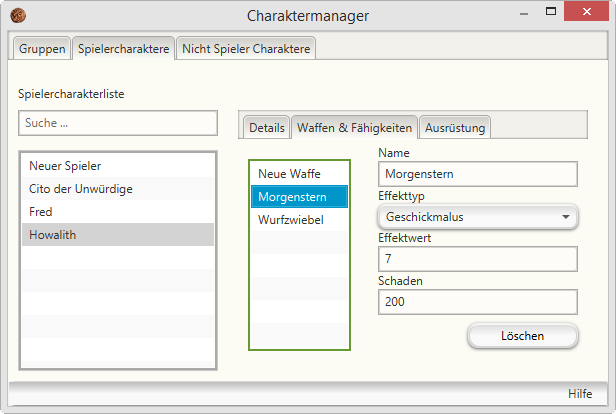
\includegraphics[width=1\linewidth]{Bilder/Charaktermanager_Spieler1}
\caption{Der Waffen\&Fähigkeiten-Tab}
\label{fig:Charaktermanager_Spieler1}
\end{figure}

Jede Waffe kann neben einen Namen und einem Schadenwert auch einen Effekt besitzen. Dafür wird zunächst der Effekttyp ausgewählt und dann der Effektwert definiert. Die Bedeutung des Effektwerts hängt vom Effekttyp ab (siehe Abschnitt \ref{Abschnitt: Effekte}): \begin{itemize}
\item[] \textit{Rüstungsunabhängig} benötigt keinen Effektwert.
\item[] \textit{Stärkemalus} spezifiziert einen absoluten Wert, der von der Stärke des Gegners subtrahiert wird.
\item[] \textit{Geschickmalus} spezifiziert einen absoluten Wert, der vom Geschick des Gegners subtrahiert wird.
\item[] \textit{Schaden an allen Gegnern} benötigt keinen Effektwert.
\end{itemize}

\textbf{Ausrüstung}: Hier wird die Rüstung des Spielercharakters spezifiziert. Dies beinhaltet natürlich den Rüstungs-, Helm- und Schildwert. Zusätzlich kann die Rüstung Effekte verursachen. Wie bei Waffen können Geschick- und Stärkemalus eingetragen werden. Hat die Rüstung keinen solchen Malus, entspricht diese einem Wert von 0. Zusätzlich kann die Rüstung eines Spielers ihm mehr Erfahrung im Kampf einbringen. Diese Steigerung wird in Prozent angegeben und später im Kampfende gesondert angezeigt.\\ %TODO::Link zu Kampfendetab
\begin{figure}
\centering
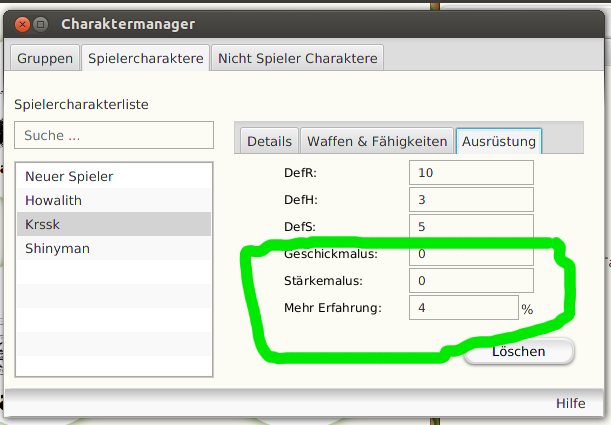
\includegraphics[width=1\linewidth]{Bilder/Spielercharaktermanager3}
\caption{Der Ausrüstungstab}
\label{fig:Spielercharaktermanager3}
\end{figure}

In jedem Tab führt ein Druck auf die 'Enter'-Taste zur Speicherung der Charakterwerte.


\subsubsection{Effekte von Rüstung und Waffen} \label{Abschnitt: Effekte}


\subsection{Der Nichtspieler-Typ-Manager}
Im Nichtspieler-Typ-Manager werden potentielle Gegner der Abenteuergruppen verwaltet. \\

Von der Bedienung her funktioniert der Nichtspieler-Typ-Manager fast identisch zum Spielermanager, siehe Abschnitt \ref{subsection:Spielercharaktermanager}. Er besitzt lediglich andere Tabs und eine zusätzliche Filterfunktion.\\

Mithilfe der Filterfunktion ist es leicht möglich, Nichtspieler-Typen eines bestimmten Kreises zu finden: Es werden stets die Typen angezeigt, deren Kreise ausgewählt sind, siehe Abbildung \ref{fig:Nichtspielertypmanager1}.
\begin{figure}
\centering
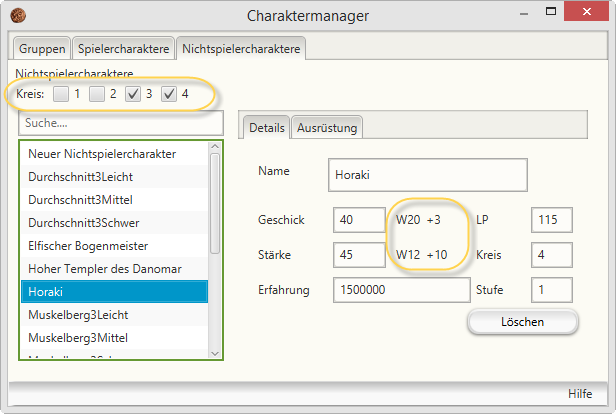
\includegraphics[width=1\linewidth]{Bilder/Nichtspielertypmanager1}
\caption{Der Nichtspieler-Typ-Manager}
\label{fig:Nichtspielertypmanager1}
\end{figure}


\subsubsection{Die zwei Untertabs für Nichtspieler-Typen-Eigenschaften}
Da für Nichtspieler-Typen im Kampf andere Werte wichtig sind, hat der Nichtspieler-Typ-Manager nur die beiden Tabs 'Details' und 'Ausrüstung'.\\

Der Tab \textbf{Details} enthält wie bei den Spielercharakteren Name, Stufe und Kreis des Typs. Auch hier kann ein Typ gelöscht werden. 
Zusätzlich können die Werte Geschick, Stärke, Erfahrung und LP gesetzt werden.\\
 Geschick und Stärke bestimmen, wie sich der Gegner im Kampf verhält. Wenn eine dieser Zahlen durch 'Enter' bestätigt wird, updaten sich auch die daneben angezeigten Würfel. 
Sie zeigen an, welche Würfelwürfe intern simuliert werden. LP bestimmt die Lebenspunkte eines Gegnertyps, Erfahrung gibt an, wie viele Erfahrungspunkte eine Instanz dieses Typs einbringt.\\
\begin{figure}
\centering
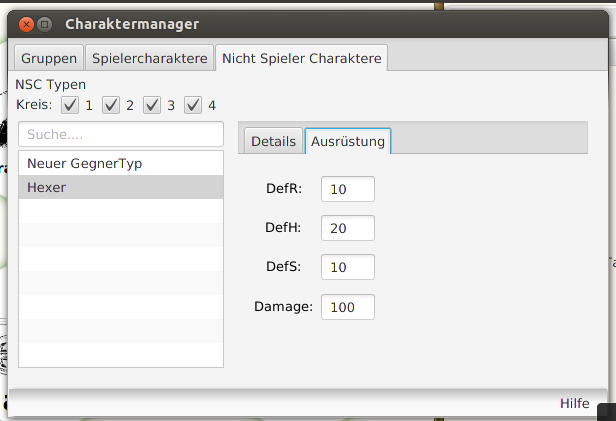
\includegraphics[width=1\linewidth]{Bilder/Nichtspielertypmanager2}
\caption{Der Ausrüstung-Tab}
\label{fig:Nichtspielertypmanager2}
\end{figure}

Im \textbf{Ausrüstung}-Tab werden erneut DefR, DefH und DefS angegeben, siehe Abschnitt \ref{subsection:Spielercharaktermanager}. 
Da einem Gegnertyp eine feste Waffe zugewiesen ist, wird hier zudem der Schaden dieser Waffe festgelegt. Effekte auf Nichtspieler-Typ-Seite sind in \textit{DLVC Taverne}, Version 1, noch nicht verfügbar.

\section{Der Kampf}
\subsection{Die Gegnerrunde}
\subsection{Die Spielerrunde}
\subsection{Das Kampfende}

\section{Der Händler}
\subsection{Allgemein}
\subsection{Inventar}
\subsection{Rüstung und Waffen}

\section{Würfeln}


\end{document}